\documentclass{standalone}
\usepackage{tikz}
\usetikzlibrary{shapes.geometric, arrows, positioning}

\begin{document} 
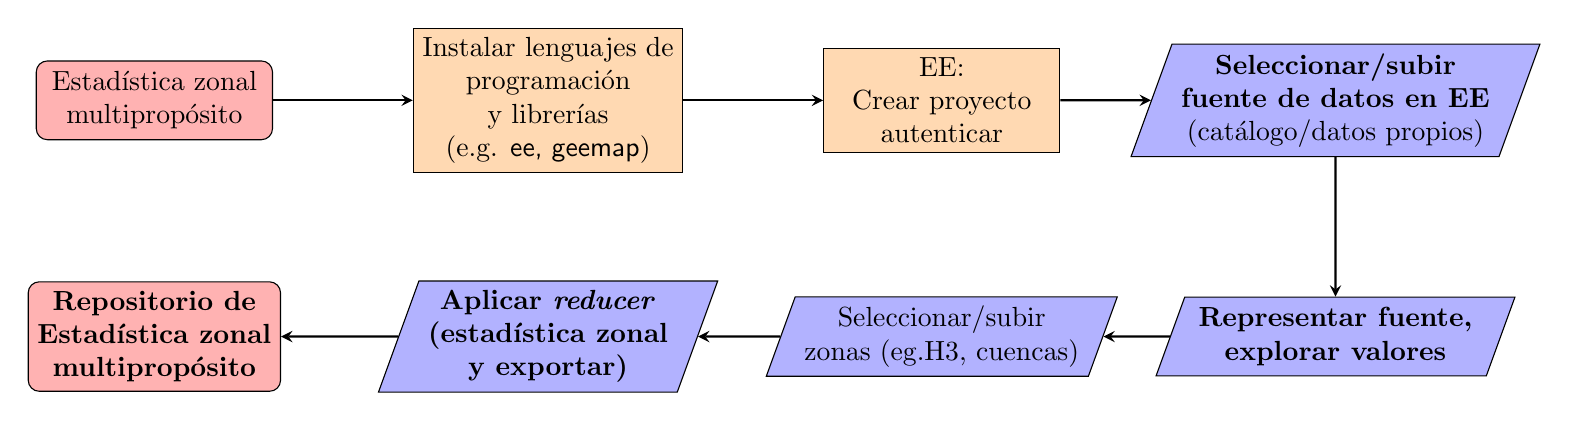
\begin{tikzpicture}[
  startstop/.style={rectangle, rounded corners, minimum width=3cm, minimum height=1cm,text centered, align=center, draw=black, fill=red!30},
  io/.style={trapezium, trapezium left angle=70, trapezium right angle=110, minimum width=3cm, minimum height=1cm, text centered, align=center, draw=black, fill=blue!30},
  process/.style={rectangle, minimum width=3cm, minimum height=1cm, text centered, align=center, draw=black, fill=orange!30},
  decision/.style={diamond, minimum width=3cm, minimum height=1cm, text centered, align=center, draw=black, fill=green!30},
  arrow/.style={thick,->,>=stealth}]

  % Nodes
  \node (start) [startstop] {Estadística zonal \\ multipropósito};
  \node (instalar) [process, right of=start, xshift=4cm] {Instalar lenguajes de \\ programación \\ y librerías \\ (e.g. \textsf{ee, geemap})};
  \node (autenticar) [process, right of=instalar, xshift=4cm] {EE: \\ Crear proyecto \\ autenticar};
   \node (fuente) [io, right of=autenticar, xshift=4cm] {\textbf{Seleccionar/subir} \\ \textbf{fuente de datos en EE} \\ (catálogo/datos propios)};

   \node (representarfuente) [io, below of=fuente, yshift=-2cm] {\textbf{Representar fuente,} \\ \textbf{explorar valores}};
   \node (zonas) [io, left of=representarfuente, xshift=-4cm] {Seleccionar/subir \\ zonas (eg.H3, cuencas)};
   \node (reducer) [io, left of=zonas, xshift=-4cm] {\textbf{Aplicar \textit{reducer}} \\ \textbf{(estadística zonal} \\ \textbf{y exportar)}};
  \node (end) [startstop, left of=reducer, xshift=-4cm] {\textbf{Repositorio de} \\ \textbf{Estadística zonal} \\ \textbf{multipropósito}};

  % Arrows
  \draw [arrow] (start) -- (instalar);
  \draw [arrow] (instalar) -- (autenticar);  
  \draw [arrow] (autenticar) -- (fuente);
  \draw [arrow] (fuente) -- (representarfuente);
  \draw [arrow] (representarfuente) -- (zonas);
  \draw [arrow] (zonas) -- (reducer);
  \draw [arrow] (reducer) -- (end);

\end{tikzpicture}
\end{document}
